%label:"fig:ChekanovTorus"
%type:"figure"
%name:" Chekanov torus"
%caption:"Chekanov Torus constructed via Lefschetz fibration"
%parent:"art_lefschetzExpanded"


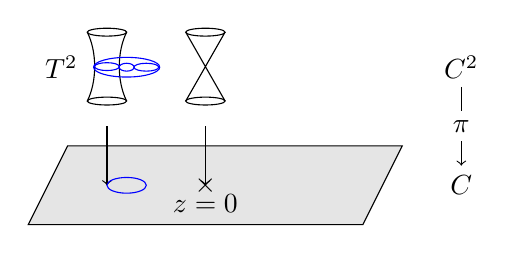
\begin{tikzpicture}[scale=.5]

\draw[fill=gray!20] (-2.5,2.5) -- (-3.5,0.5) -- (5,0.5) -- (6,2.5) -- cycle;
\begin{scope}[scale=0.5, shift={(6,3.78)}]
\draw  (-4,7) ellipse (1 and 0.2);
\draw  (-4,3.5) ellipse (1 and 0.2);
\draw (-5,7) -- (-3,3.5) (-5,3.5) -- (-3,7);
\end{scope}

\begin{scope}[scale=0.5,shift={(1,3.78)}]
\draw  (-4,7) ellipse (1 and 0.2);
\draw  (-4,3.5) ellipse (1 and 0.2);

\draw (-5,7) .. controls (-4.5,6) and (-4.5,4.5) .. (-5,3.5);
\draw (-3,7) .. controls (-3.5,6) and (-3.5,4.5) .. (-3,3.5);
\draw[blue]  (-4,5.25) ellipse (0.63 and 0.2);
\end{scope}

\draw[->] (-1.5,3) -- (-1.5,1.5);
\draw[->](1,3) -- (1,1.5);
\node at (1,1.5) {$\times$};
\node[below] at (1,1.5) {$z=0$};


\node at (7.5,1.5) {$\mathbb C$};
\node at (7.5,4.5) {$\mathbb C^2$};
\draw[->] (7.5,4) -- (7.5,2);
\node[fill=white] at (7.5,3) {$\pi$};





\node[left] at (-2,4.5) {$T^2$};

\draw[blue]  (-1,4.5) ellipse (0.19 and 0.1);
\draw[blue, scale=.5]  (-1,9) ellipse (0.63 and 0.2);
\draw[blue]  (-1,4.5) ellipse (.84 and 0.25);
\draw[blue]  (-1,1.5) ellipse (0.5 and 0.2);

\end{tikzpicture}